%-----------------------------------------------------------------
% TITLE PAGE
%-----------------------------------------------------------------
	% deactivate header and footer
	\pagestyle{superempty}
	
    % set geometry and create black area for thumbtabs
	\fronttitleprep%

	% title blocks
	\begin{tikzpicture}[overlay, remember picture]
		% title
		\node[
			anchor=north west,
			xshift=-5mm,
			yshift=-5mm,
			font=\Huge
		] (techcheck) at (current page text area.north west) {%
			\fontspec[
				Path=./fonts/,
				Ligatures=TeX,
				LetterSpace=5.0,
			]{Spartan MB-Light}
			Tech's Checks
		};
		\node[
			anchor=north west,
			yshift=-0.5em,
			fill=color1,
			text=white,
			minimum width=\textwidth,
			font=\huge,
		](name) at (techcheck.south west) {%
			\fontspec[
				Path=./fonts/,
				Ligatures=TeX,
			]{Spartan MB-SemiBold}%
			\aircraftlong%
		};
		\node[
			anchor=north west,
			yshift=-0.5em,
			font=\large
		] () at (name.south west) {%
			\fontspec[
				Path=./fonts/,
				Ligatures=TeX,
				LetterSpace=5.0,
			]{Spartan MB-Light}
			REV: \today
		};
		\node[
			xshift=10mm,
			yshift=0mm,
		](pic) at (current page text area.west) {%
			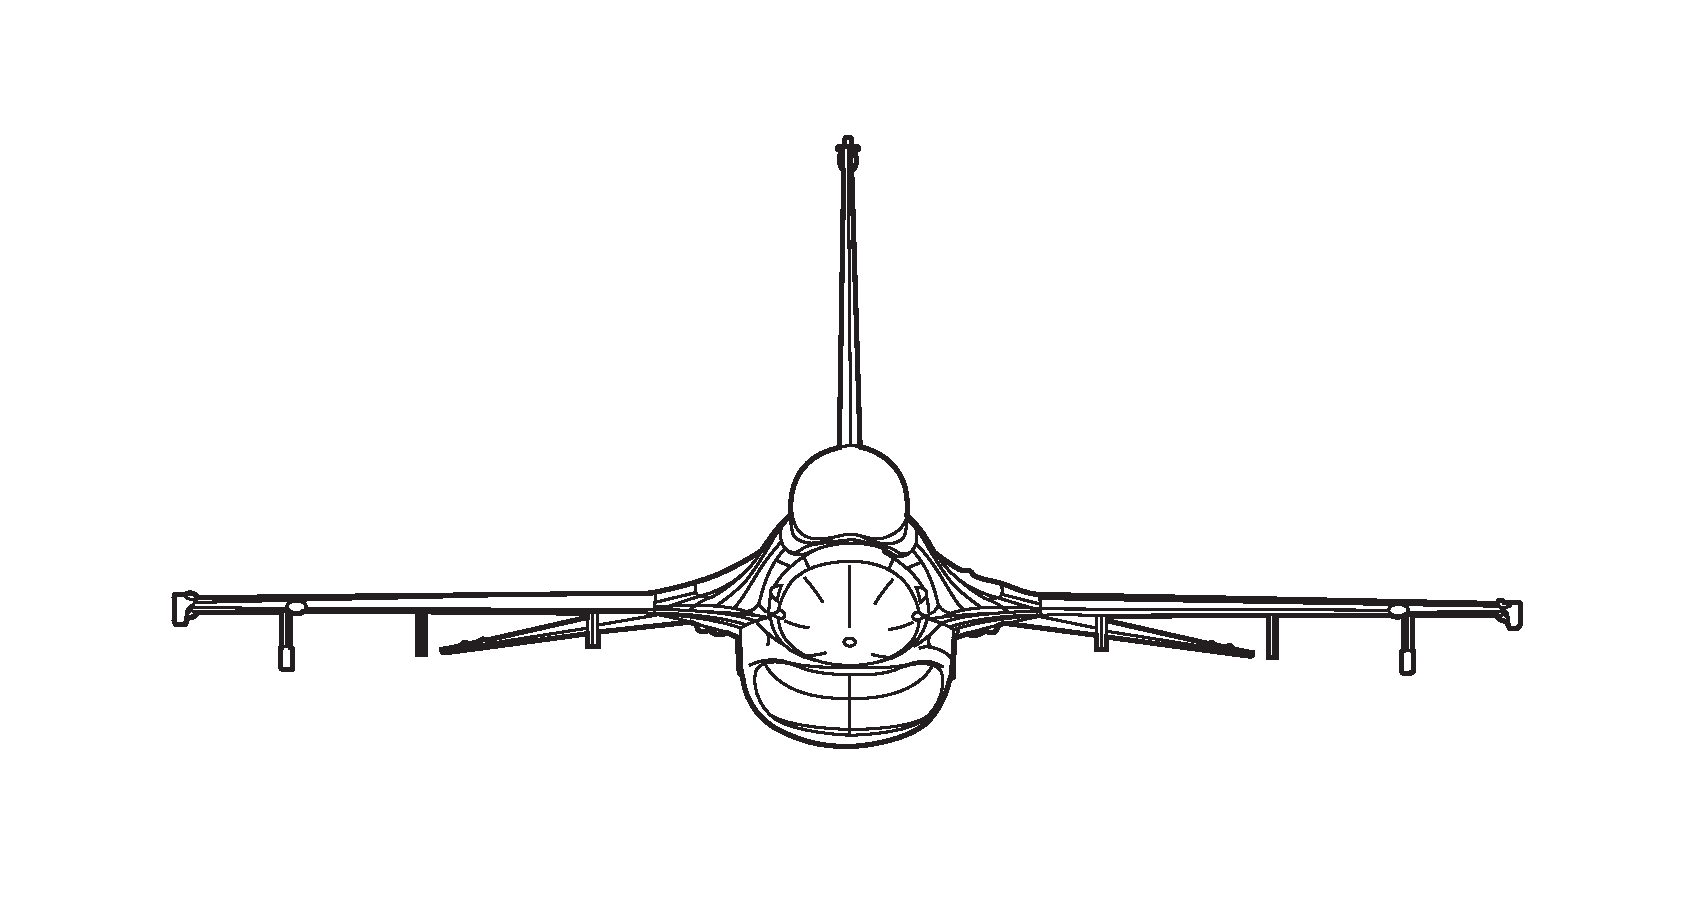
\includegraphics[%
				width=2\textwidth,%
			]{diagrams/aircraft/wireframe_front.pdf}%
		};
		% gold band for edition
		\node[
			anchor=south,
			xshift=-5mm,
			yshift=0mm,
			minimum width=\textwidth,
			font=\large,
			fill=techyellow,
		] (gold) at (current page text area.south) {%
			\fontspec[
				Path=./fonts/,
				Ligatures=TeX,
			]{Spartan MB-Medium Italic}%
			Gold Edition%
		};
		% authors
		\node[
			anchor=south east,
			xshift=-0mm,
			yshift=2em,
			font=\large,
		] (goldwolf) at (gold.north east) {
			\fontspec[
				Path=./fonts/,
				Ligatures=TeX,
			]{Spartan MB-Light Italic}%
			and Goldwolf%
		};
		\node[
			anchor=south east,
			xshift=-0mm,
			yshift=0em,
			font=\large,
		] (techneatium) at (goldwolf.north east) {
			\fontspec[
				Path=./fonts/,
				Ligatures=TeX,
			]{Spartan MB-Light Italic}
			By Techneatium%
		};
	\end{tikzpicture}

	% label for hyperrefs back to frontpage
	\label{frontpage}
	% make thumbfronts
	\thumbfront{Procedures \\ {\footnotesize Normal}}{0}{1}
	\cyclechpcolor%
	\thumbfront{Procedures \\ {\footnotesize Emergency}}{1}{2}
	\cyclechpcolor%
	\thumbfront{Aircraft \\ Systems}{2}{3}
	\cyclechpcolor%
	\thumbfront{Sensors \\ {\footnotesize A-A}}{3}{4}
	\cyclechpcolor%
	\thumbfront{Sensors \\ {\footnotesize A-G}}{4}{5}
	\cyclechpcolor%
	\thumbfront{Weapons \\ {\footnotesize A-G}}{5}{6}
	\cyclechpcolor%
	\thumbfront{Weapons \\ {\footnotesize A-A}}{6}{7}
	\cyclechpcolor%
	\thumbfront{Appendix}{7}{A}
	\thumbwide%

    \restoregeometry
	\clearpage

	\begin{tikzpicture}[overlay, remember picture]
		% logos
		\node[
			anchor=center,
			xshift=-\textwidth/4,
			yshift=-40mm,
		](logotc) at (current page text area.north) {%
			\IfFileExists{%
				figs/diagrams/logos/techschecks.pdf%
			}{%
				\includegraphics[%
					height=\textwidth/3,%
					page=1,%
				]{diagrams/logos/techschecks.pdf}%
			}{}%
		};
		\node[
			anchor=center,
			xshift=\textwidth/4,
			yshift=-40mm,
		](logogoldwolf) at (current page text area.north) {%
			\IfFileExists{%
				figs/diagrams/logos/goldwolf.pdf%
			}{%
				\includegraphics[%
					height=\textwidth/3,%
					page=1,%
				]{diagrams/logos/goldwolf.pdf}%
			}{}%
			
		};
		% cc
		\node[
			anchor=south west,
			xshift=0mm,
			yshift=0mm,
			minimum width=\textwidth/1.5,
			text width=\textwidth/1.5,
			font=\normalsize,
			align=left,
		] (cc) at (current page text area.south west) {%
			\fontspec[
				Path=./fonts/,
				Ligatures=TeX,
				LetterSpace=5.0,
			]{Spartan MB-Light Italic}
			The figures and illustrations contained within this work are licensed under 
			\href{http://creativecommons.org/licenses/by-sa/4.0/}{CC BY-SA 4.0}.
		};
		% thanks
		\node[
			anchor=south west,
			xshift=0mm,
			yshift=2em,
			minimum width=\textwidth/1.5,
			text width=\textwidth/1.5,
			font=\normalsize,
			align=left,
		] (thanks) at (cc.north west) {%
			\fontspec[
				Path=./fonts/,
				Ligatures=TeX,
				LetterSpace=5.0,
			]{Spartan MB-Light Italic}
			Special thanks to \hfill\\
			\hfill Mythic \\
			\hfill TheMerryMarlin \\
			\hfill The UOAF Community
		};
		\node[
			anchor=south west,
			xshift=0mm,
			yshift=2em,
			minimum width=\textwidth/1.5,
			text width=\textwidth/1.5,
			font=\large,
			align=left,
		] (morkvitnir) at (thanks.north west) {%
			\fontspec[
				Path=./fonts/,
				Ligatures=TeX,
				LetterSpace=5.0,
			]{Spartan MB-Italic}
			Custom typefaces by \hfill\\
			\hfill Morkvitnir
		};
	\end{tikzpicture}
	\cleardoublepage
	\resetchpcolor
